% \textbf{\underline{OZ 6 - Magnetische inductie en de wet van Faraday - Oefening 4:}}
% \vspace{0.5cm}

% Een rechthoekige loop met dimensies $ l $ en $ w $ beweegt met een constante snelheid $ v $ weg van een lange rechte draad waardoor een stroom $ I $ loopt, zoals aangeven op Figuur 6.4. De totale weerstand van de loop is $ R $. Bepaal een uitdrukking dat de stroom in de loop als een functie van de afstand $ r $.

% \begin{figure}[H]
%     \centering
%     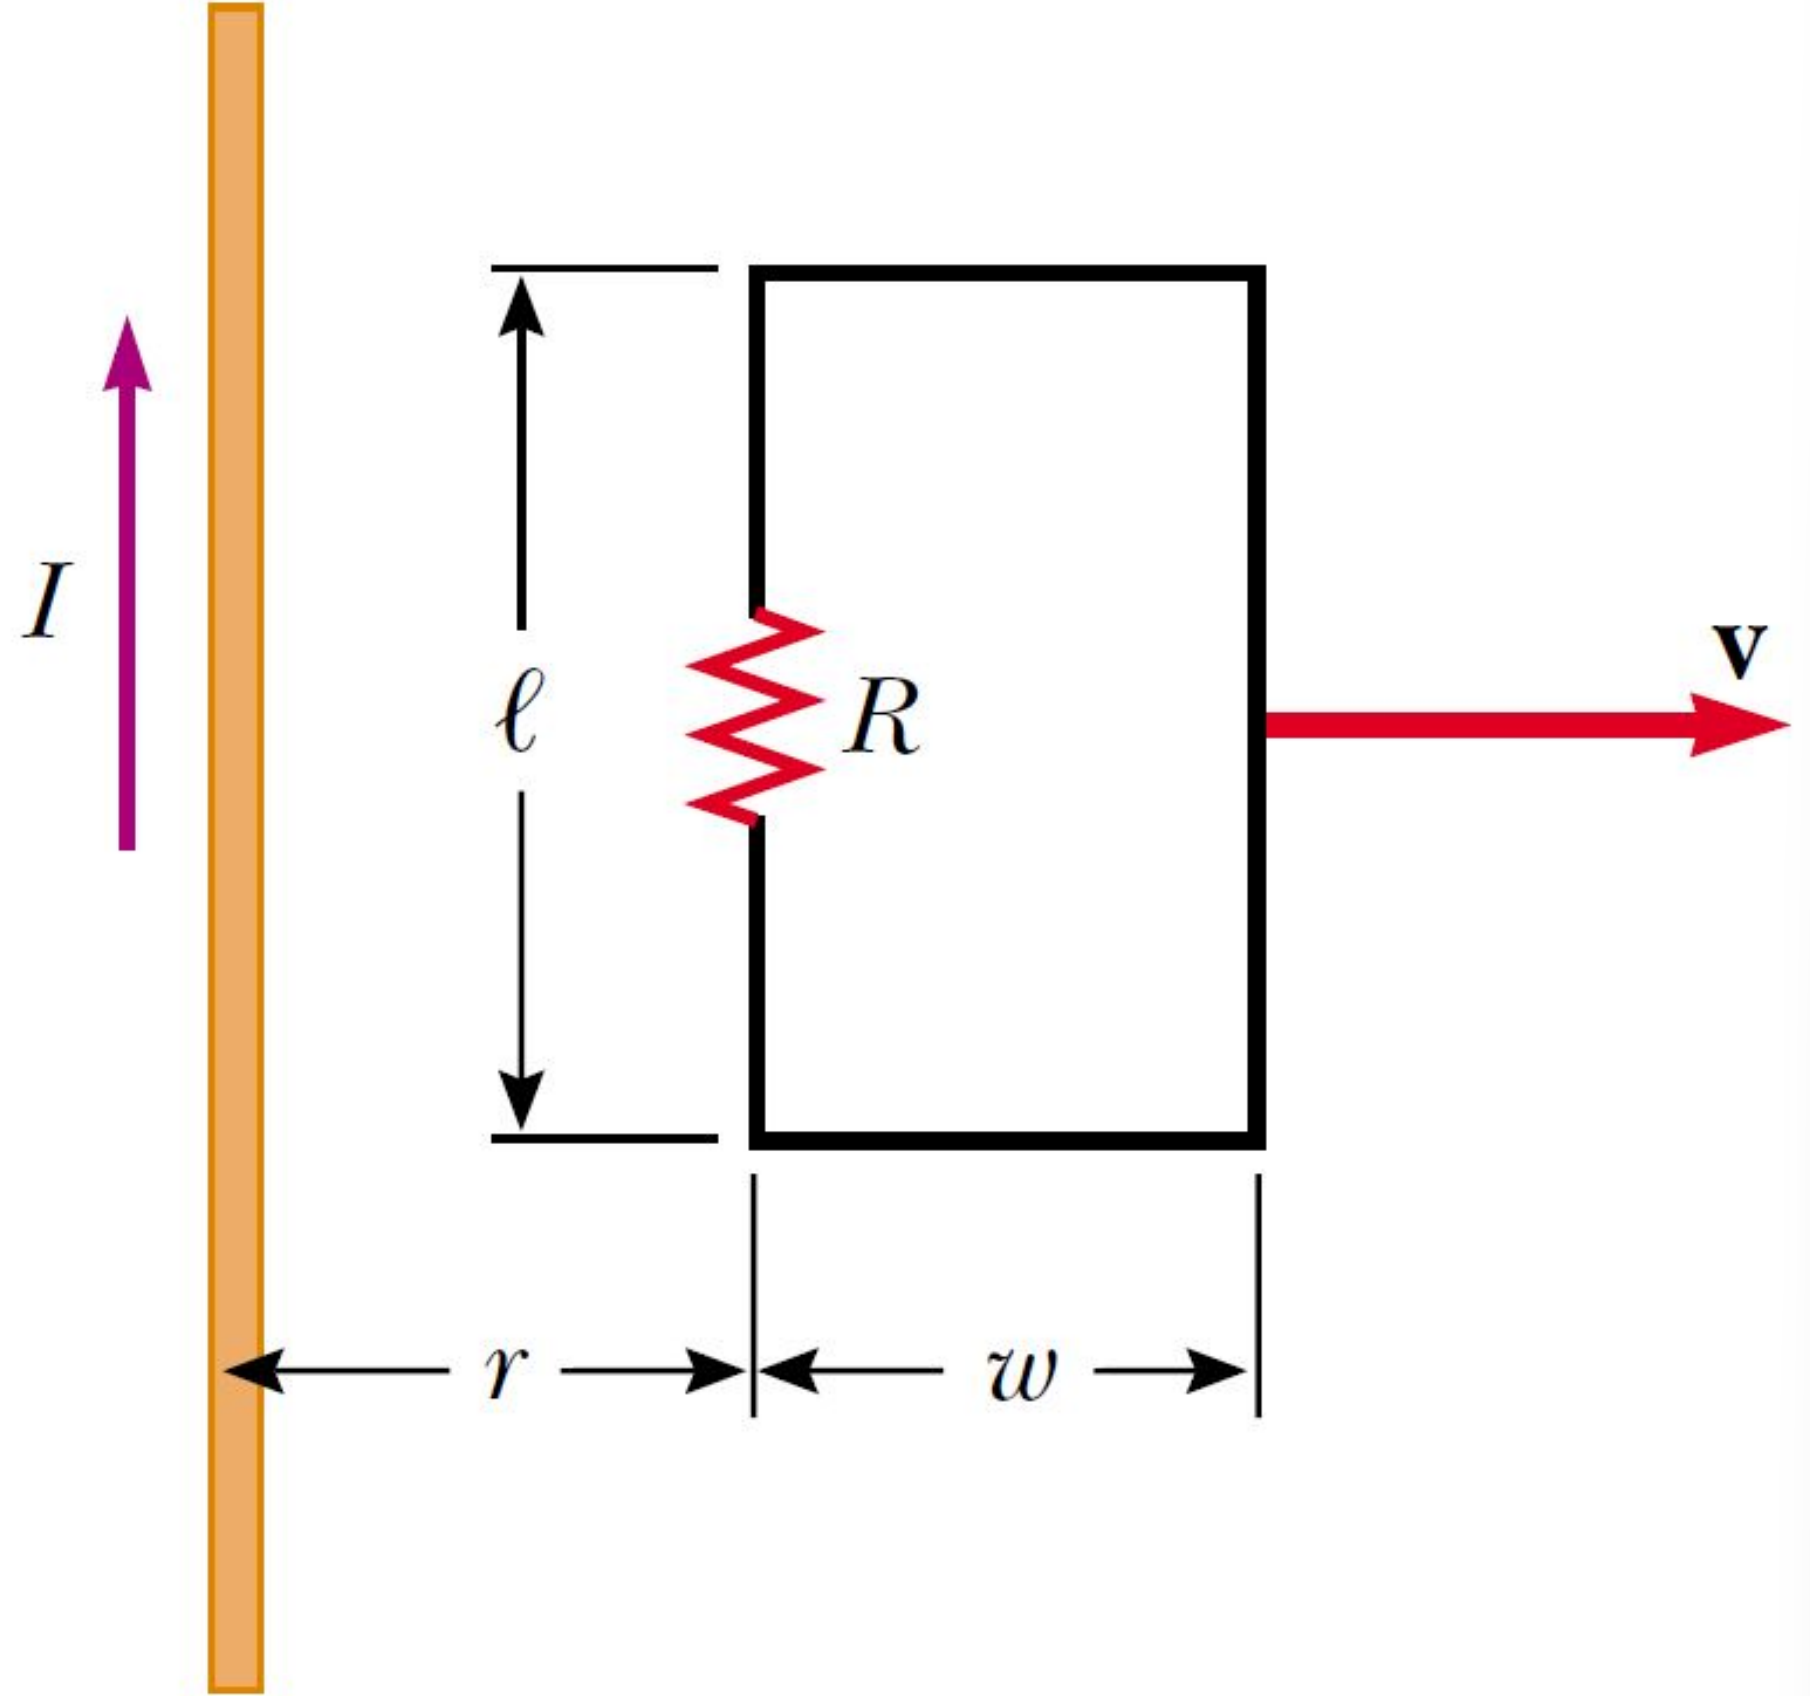
\includegraphics[width=5cm]{oz06/resources/oef-4-opgave.png}
    
%     \textbf{Figuur 6.4}
% \end{figure}

% \begin{description}[labelwidth=1.5cm, leftmargin=!]
%     \item[Geg. :]   $ l $; $ w $; $ v $; $ I $; $ R $;
%     \item[Gevr. :]  $ I_{l}(r) $;
%     \item[Opl. :]   $ B = \dfrac{\mu_0 I}{2 \pi r} $
                    
%                     $ \Phi_B = \int{\vec{B} \cdot d\vec{A}} = \int{\dfrac{\mu_0 I}{2 \pi r} \cdot l \cdot dr} $
                    
%                     \hspace{-0.57cm} $ \Rightarrow 
%                     \Phi_B = \dfrac{\mu_0 I l}{2 \pi} \int_{r}^{r+w}{\dfrac{dr}{r}} 
%                     = \dfrac{\mu_0 I l}{2 \pi} \left( \ln{\left| r+w \right|} - \ln{\left| r \right|} \right) 
%                     = \dfrac{\mu_0 I l}{2 \pi} \ln{\dfrac{r+w}{r}} 
%                     = \dfrac{\mu_0 I l}{2 \pi} \ln{\left( 1 + \dfrac{w}{r} \right)} $
                    
%                     \vspace{0.5cm}
                    
%                     $ r = r_0 + vt $
                    
%                     \vspace{0.5cm}
                    
%                     \hspace{-0.57cm} $ \Rightarrow 
%                     \Phi_B = \dfrac{\mu_0 I l}{2 \pi} \ln{\left( 1 + \dfrac{w}{r_0 + vt} \right)} $
                    
%                     \hspace{-0.57cm} $ \Rightarrow 
%                     \dfrac{d\Phi_B}{dt} = \dfrac{\mu_0 I l}{2 \pi} \dfrac{1}{1 + \dfrac{w}{r_0 + vt}} \dfrac{d}{dt}{\left( 1 + \dfrac{w}{r_0 + vt} \right)}
%                     = \dfrac{\mu_0 I l}{2 \pi} \dfrac{1}{1 + \dfrac{w}{r_0 + vt}} \dfrac{d}{dt}{\left( 1 + \dfrac{w}{r_0 + vt} \right)} $
                    
%                     \hspace{0.75cm} $ 
%                     = \dfrac{\mu_0 I l}{2 \pi} \dfrac{w}{1 + \dfrac{w}{r_0 + vt}} \dfrac{d}{dt}{\left( \dfrac{1}{r_0 + vt} \right)}
%                     = \dfrac{\mu_0 I l}{2 \pi} \dfrac{w}{1 + \dfrac{w}{r_0 + vt}} \dfrac{1}{\left( r_0 + vt \right)^2} \dfrac{d}{dt}{\left( r_0 + vt \right)}$
                    
%                     \hspace{0.75cm} $ 
%                     = \dfrac{\mu_0 I l}{2 \pi} \dfrac{w}{1 + \dfrac{w}{r_0 + vt}} \dfrac{v}{\left( r_0 + vt \right)^2}
%                     = \dfrac{\mu_0 I l}{2 \pi} \dfrac{w}{1 + \dfrac{w}{r}} \dfrac{v}{r^2} 
%                     = \dfrac{\mu_0 I l v}{2 \pi r} \dfrac{w}{r + w} $
                    
%                     $ \varepsilon = -\dfrac{d\Phi_B}{dt} = -\dfrac{\mu_0 I l v}{2 \pi r} \dfrac{w}{r + w} $
                    
%                     $ I = \dfrac{\varepsilon}{R} = -\dfrac{\mu_0 I l v}{2 \pi R r} \dfrac{w}{r + w} $
% \end{description}

% \vspace{1cm}